% Created 2023-09-10 Sun 20:59
% Intended LaTeX compiler: pdflatex
\documentclass[12pt, a4paper]{article}
\usepackage[utf8]{inputenc}
\usepackage[T1]{fontenc}
\usepackage{graphicx}
\usepackage{longtable}
\usepackage{wrapfig}
\usepackage{rotating}
\usepackage[normalem]{ulem}
\usepackage{amsmath}
\usepackage{amssymb}
\usepackage{capt-of}
\usepackage{hyperref}
\usepackage{placeins}
\usepackage{gensymb}
\usepackage[letterpaper]{geometry}
\geometry{top=1.0in, bottom=1.0in, left=1.0in, right=1.0in}
\usepackage{rotating}
\usepackage{graphicx}
\usepackage{fancyhdr}
\usepackage{pgfplots}
\usepackage{filecontents}
\usepackage{tikz}
\pagestyle{fancy}
\lhead{}
\chead{}
\rhead{Johnson \thepage}
\lfoot{}
\cfoot{}
\rfoot{}
\renewcommand{\headrulewidth}{0pt}
\renewcommand{\footrulewidth}{0pt}
\setlength\headsep{0.333in}
\newcommand{\bibent}{\noindent \hangindent 40pt}
\newenvironment{workscited}{\newpage \begin{center} Works Cited \end{center}}{\newpage }
\graphicspath{ {./attachments/} }
\author{Christian Johnson}
\date{\today}
\title{Lab 0 Report}
\hypersetup{
 pdfauthor={Christian Johnson},
 pdftitle={Lab 0 Report},
 pdfkeywords={},
 pdfsubject={},
 pdfcreator={Emacs 28.2.50 (Org mode 9.7-pre)}, 
 pdflang={English}}
\begin{document}

\begin{document}
\begin{flushleft}
Christian Johnson\\
\vspace{2mm}
Dr. Paul Crilly\\
\vspace{2mm}
Antennas and Propogation\\
\vspace{2mm}
September 06 2023\\
\vspace{4mm}
\begin{center}
\Large{\textbf{\underline{Lab 0 Report}}}
\end{center}
\vspace{1mm}
\setlength{\parindent}{0.5in}

\begin{abstract}

This laboratory assignment aimed to analyze the behavior of high-frequency signals at different times of the day, focusing on frequencies ranging from 2.5 MHz to 15 MHz. Our goal was to qualitatively assess signal strength variations, identify trends, and extrapolate the impact of ionospheric layers on radio communication. We placed particular emphasis on the influence of sunrise and sunset on signal propagation, recognizing their significance in radio communication. In summary, this study enhances our understanding of HF communication dynamics.

\newline
\end{abstract}
\section*{Procedures}
\label{sec:org1f164f6}

In this experiment, we sought to explore high-frequency (HF) signals and their interactions with ionosphere layers, particularly the E and F layers. Our study involved tracking NIST broadcast signals over a span of approximately 12 hours, monitoring the clarity with which we received these signals in New London, CT. To achieve this, we followed a well-defined series of procedures, helping us gain an insight into HF wave behavior under varying conditions.
Using a Kenwood receiver located in Macallister Hall room 213, we conducted hourly measurements of signal strength and clarity for four distinct frequencies: 2.5, 5, 10, and 15 MHz. Our goal was to capture data over a continuous 12-hour period; however, due to academic commitments and scheduling constraints, we divided this observation period into two days. We recorded data from 1300 to 2100 hours on August 29, 2023, and from 0500 to 0700 hours on September 1, 2023. Measurements were graded on a scale from zero to three: Three indicated a perfectly clear signal, where both voice and carrier were audible; Two represented a state in which both components were audible but not clearly discernible. One signified a minimal signal, with only the carrier being audible and no discernible voice. Zero indicated a completely undetectable signal, where neither carrier nor voice were audible.
To ensure the accuracy and consistency of our data, we maintained a strict measurement schedule, striving to record readings as close to the top of each hour as possible. Furthermore, we adhered to a one-minute adjustment period before each measurement, allowing our ears to acclimate to the signal conditions. Following these procedures, we were able to collect consistent data that was relatively easy to analyze and interpret, allowing us to draw logical conclusions from the information we recorded.
\section*{Results}
\label{sec:orgd2766dd}

Our investigation into high-frequency (HF) radio signal propagation encompassed data collection over two days, totaling approximately 11 hours. The recorded dataset (shown below) reflects signal strength observations at four frequencies: 2.5 MHz, 5 MHz, 10 MHz, and 15 MHz.


\begin{table}[htbp]
\begin{center}
\caption{Signal Strength Measurements}
\label{tab:signal-strength}
\begin{tabular}{|c|c|c|c|c|c|}
\hline
\multicolumn{1}{|c|}{\textbf{Date}} & \multicolumn{1}{c|}{\textbf{Time}} & \multicolumn{1}{c|}{\textbf{2.5 MHz}} & \multicolumn{1}{c|}{\textbf{5 MHz}} & \multicolumn{1}{c|}{\textbf{10 MHz}} & \multicolumn{1}{c|}{\textbf{15 MHz}} \\ \hline
\multirow{August 29, 2023} & 1300 & 0 & 0 & 1 & 2 \\ \cline{2-6} 
 & 1400 & 0 & 0 & 1 & 2 \\ \cline{2-6} 
 & 1500 & 0 & 0 & 1 & 1 \\ \cline{2-6} 
 & 1600 & 0 & 0 & 1 & 1 \\ \cline{2-6} 
 & 1700 & 0 & 0 & 1 & 2 \\ \cline{2-6} 
 & 1800 & 0 & 0 & 1 & 1 \\ \cline{2-6} 
 & 1900 & 0 & 0 & 2 & 3 \\ \cline{2-6} 
 & 2000 & 0 & 0 & 2 & 3 \\ \cline{2-6}
 & 2100 & 0 & 2 & 2 & 3 \\ \hline
\multirow{September 1, 2023} & 0500 & 1 & 3 & 2 & 2 \\ \cline{2-6} 
 & 0600 & 1 & 2 & 2 & 1 \\ \cline{2-6} 
 & 0700 & 0 & 2 & 1 & 2 \\ \hline
\end{tabular}
\end{center}
\end{table}

Throughout the afternoon hours, the signal strength at 2.5 MHz stayed consistently low. It improved slightly during the early hours, peaking at 1 from 0500 to 0600 with the carrier being faintly audible. As the day went on and the sun began to rise however, it sank back down to a 0. Similarly, the 5 MHz signal was inaudible from 1300-2000, jumping up to a 2 as the sun sank at 2100, and reaching 3 at 0500. The 10 MHz signal remained relatively constant, the carrier audible consistently from 1300 to 2100, the speaker fading in from 1900 onward. On the other hand, the 15 MHz signal was somewhat sporadic; the carrier was audible during every test, but the speakers voice seemed to face in and out. There did seem to be a general trend, with each signal seeming fainter during the daylight hours, and growing stronger at night. In order to support this theory, we recorded sunrise and sunset times for our location in New London CT, and for the location of the NIST broadcast station in Fort Collins CO. This data in shown below.

\begin{table}[htbp]
\centering
\caption{Sunrise and Sunset Times}
\label{tab:sunrise-sunset}
\begin{tabular}{|c|c|c|c|c|}
\hline
\multicolumn{1}{|c|}{\textbf{Location}} & \multicolumn{1}{c|}{\textbf{Date}} & \multicolumn{1}{c|}{\textbf{Sunrise (EST)}} & \multicolumn{1}{c|}{\textbf{Sunset (EST)}} \\ \hline
\multirow{New London} & August 29, 2023 & 0611 & 1926 \\ \cline{2-4} 
 & September 1, 2023 & 0614 & 1921 \\ \hline
\multirow{Fort Collins} & August 29, 2023 & 0823 & 2138 \\ \cline{2-4} 
 & September 1, 2023 & 0827 & 2132 \\ \hline
\end{tabular}
\end{table}

Examining the similarities between the changes in signal strength and the sunrise and sunset times for both locations, it seems as if the data we recorded shows a correlation between the time of day and the strength of the signal received. When the sun starts to fade in both locations, we see an increase in the received signal - we see this at around 2100 on the 29th. At 2000, the sun has set in New London, but is still up in Colorado. As dusk sets in Fort Collins, we see the lower frequency signals start to increase and come through more clearly. We see the inverse effect on the morning of the 1st - the sun is set in both cities at 0500, and all signals are coming through to some extent. As the sun starts to rise in New London however, the lower frequencies disappear and the higher frequencies begin to fade.



\vspace{2mm}
\begin{filecontents*}{data.txt}
Time 2.5MHz 5MHz 10MHz 15MHz
13 0 0 1 2
14 0 0 1 2
15 0 0 1 1
16 0 0 1 1
17 0 0 1 2
18 0 0 1 1
19 0 0 2 3
20 0 0 2 3
21 0 2 2 3
05 1 3 2 2
06 1 2 2 1
07 0 2 1 2
\end{filecontents*}

\begin{document}

\begin{tikzpicture}[htb]
\begin{axis}[
    title={Graph 1: Signal Strength Over Time},
    xlabel={Time},
    ylabel={Signal Strength},
    grid=major,
    legend style={at={(0.5, -0.3)},
    anchor=north,
    legend columns=4},
    xtick=data,
    xticklabel style={rotate=45,anchor=east},
    xticklabels from table={data.txt}{Label},
    ymin=0, ymax=3,
    ytick={0,1,2,3},
    yticklabels={0,1,2,3},
    width=15cm,
    height=7cm,
    unbounded coords=jump,
]

\addplot[mark=square*, olive, solid, line width=2pt] table [x expr=\coordindex, y=2.5MHz] {data.txt};
\addplot[mark=triangle*, purple, solid] table [x expr=\coordindex, y=5MHz] {data.txt};
\addplot[mark=o, orange, solid] table [x expr=\coordindex, y=10MHz] {data.txt};
\addplot[mark=diamond*, grey, solid] table [x expr=\coordindex, y=15MHz] {data.txt};

\legend{2.5MHz,5MHz,10MHz,15MHz}

% Vertical lines for sunrise and sunset with updated colors and line styles
\draw[red, solid, line width=2pt] (axis cs:3.25,0) -- (axis cs:3.25,3);
\draw[red, dashed, line width=2pt] (axis cs:12.51,0) -- (axis cs:12.51,3);
\draw[blue, solid, line width=2pt] (axis cs:1.25,0) -- (axis cs:1.25,3);
\draw[blue, dashed, line width=2pt] (axis cs:10.52,0) -- (axis cs:10.52,3);


% Add sunrise and sunset to the legend
\addlegendimage{red, solid, line width=2pt}
\addlegendentry{Sunrise CO}
\addlegendimage{red, dashed, line width=2pt}
\addlegendentry{Sunset CO}
\addlegendimage{blue, solid, line width=2pt}
\addlegendentry{Sunrise CT}
\addlegendimage{blue, dashed, line width=2pt}
\addlegendentry{Sunset CT}

\end{axis}
\end{tikzpicture}
\vspace{2mm}

Our analysis highlights a clear connection between time of day, sunset, and sunrise with HF radio signal strength. Signal quality improved as daylight decreased and vice versa. This correlation underscores the intricate interplay between HF signal propagation and ionospheric layers, providing valuable insights into radio wave behavior.
\section*{Conclusion}
\label{sec:org1a8e7a4}

Overall, our study sheds light on the dynamic nature of HF radio signal propagation, particularly how it relates to ionospheric conditions and daylight variations. By analyzing signal strength across different frequencies, we were able to observe a consistent pattern of weaker signals during daylight hours and stronger signals at night. This phenomenon aligns with our recorded sunrise and sunset times - affirming our expectations and indicating a direct link between ionospheric changes and signal clarity.

\newpage
\begin{center}
Appendices
\end{center}
\begin{figure}[htb]
\centering
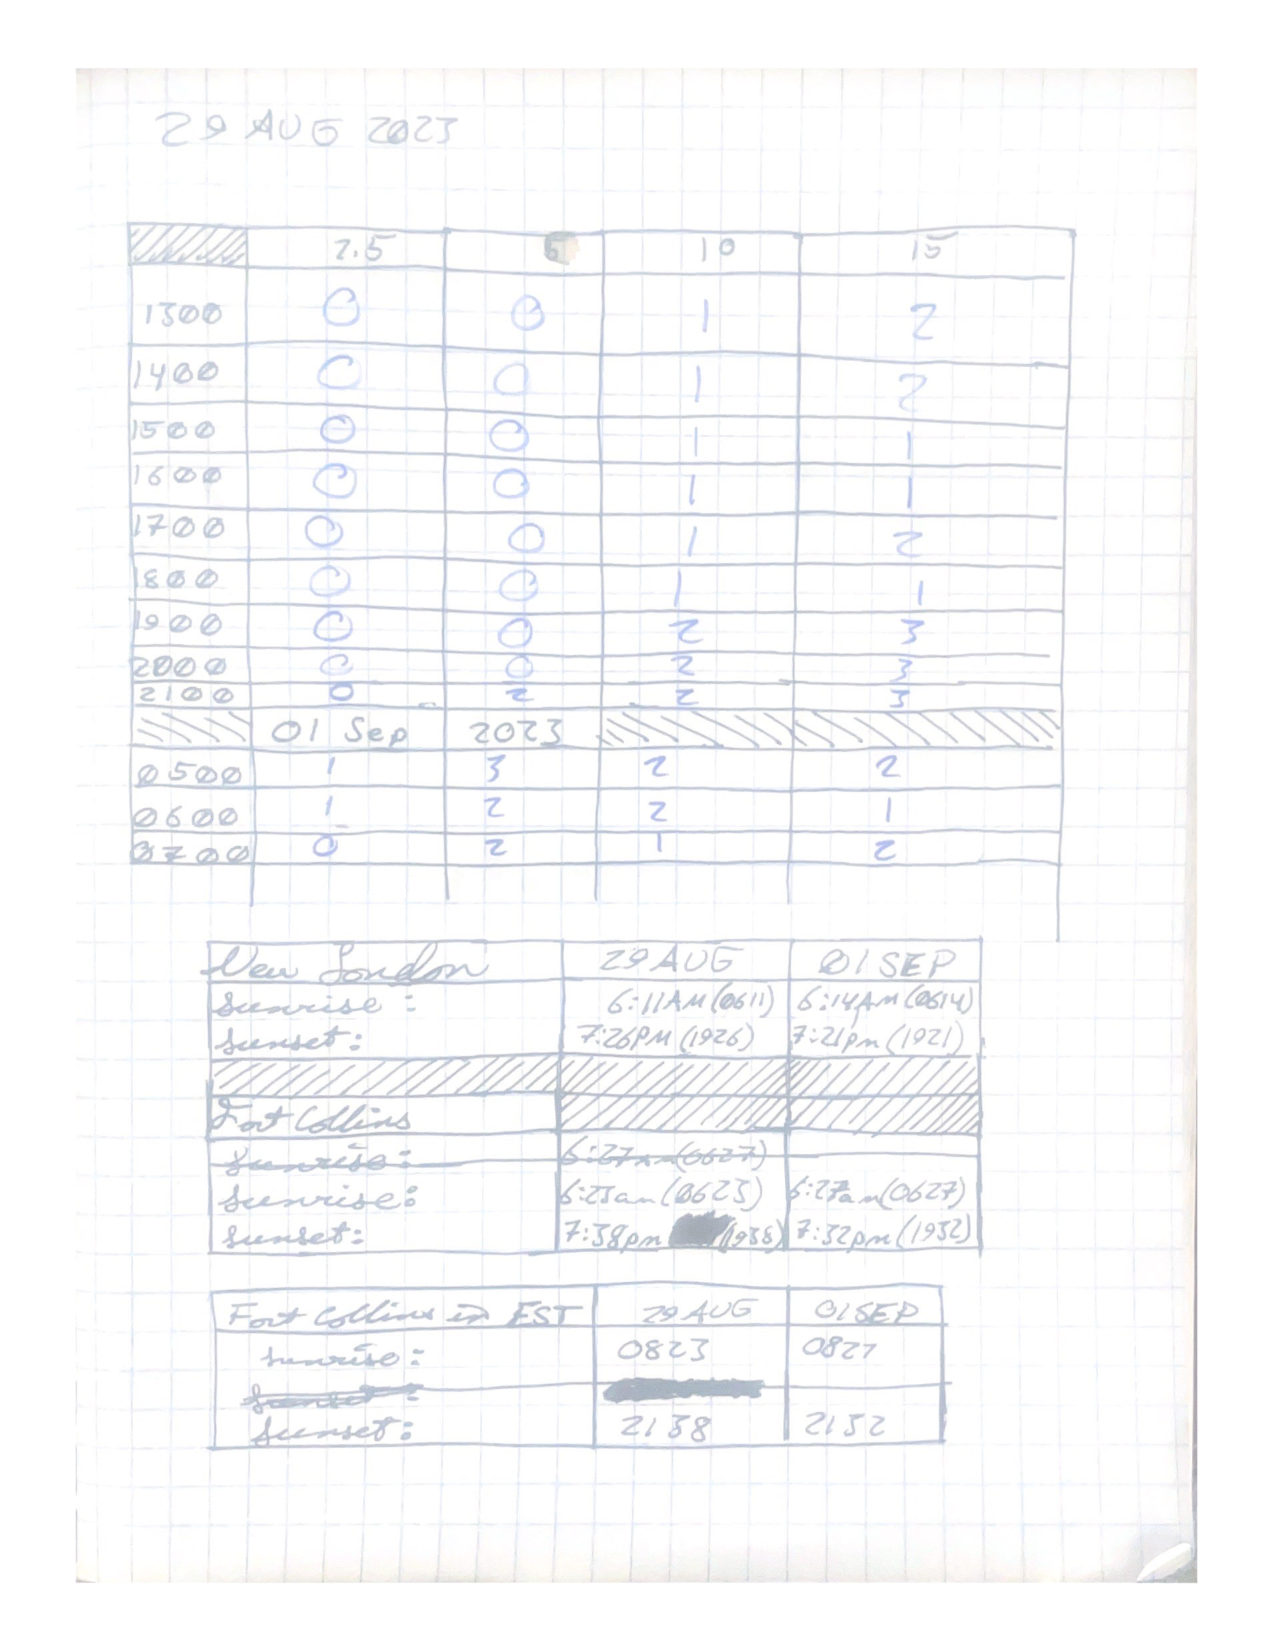
\includegraphics[width=0.7\textwidth]{Lab0 Data.pdf}
\caption{All Recorded Data}
\end{figure}

% Insert Notes in bullet-points

\newpage
\begin{center}
Lab Questions
\end{center}
\begin{enumerate}
\item I would expect the 2.5 and 5 MHz signals to cease around 1-2 hours after sunrise and begin again around 1-2 hours after sunset. This delay is due to the difference in time zones between New London and Fort Collins, and this loosely matches our data. The actual times were slightly different, possibly due to weather in each city, or other external factors.
\item Groundwave propagation involves waves traveling along the earth's surface, while skywave propagation involves signals reflecting off of layers in the ionosphere in order to travel long distances.
\item Some notable limitations to this method include susceptibility to solar radiation and weather conditions, D-layer absorption, and potential interference.
\item The Norton surface wave is used because higher frequencies have a higher rate of attenuation and cannot travel as far due to their limited groundwave propagation.
\item Ground waves can be used to communicate via surface wave propagation, and line of sight communication.
\item Operating LORAN at a higher frequency led to a more limited groundwave propagation range.
\item There are two primary ways to reduce D-layer attenuation - namely, waiting until nightfall, or using higher-frequency signals.
\item The 10 meter band is used primarily to increase bandwidth (more information can be transmitted) and to reduce attenuation in the atmosphere.
\end{enumerate}

\end{document}
\end{document}